\section{Структура опросов}\label{sec:-}

\subsection{Основной опрос}\label{subsec:-}

Опрос представляет собой дерево.
В зависимости от данного человеком ответа, будет подбираться следующий вопрос.
Вопросы разбиваются на блоки.
Каждый ответ на вопрос имеет свою ценность в виде баллов.
Если при ответе на вопросы пациент набрал N-ное количество баллов и более для данного блока, то это означает, что его здоровье ухудшилось и стоит обратиться к врачу.

\begin{figure}[h]
    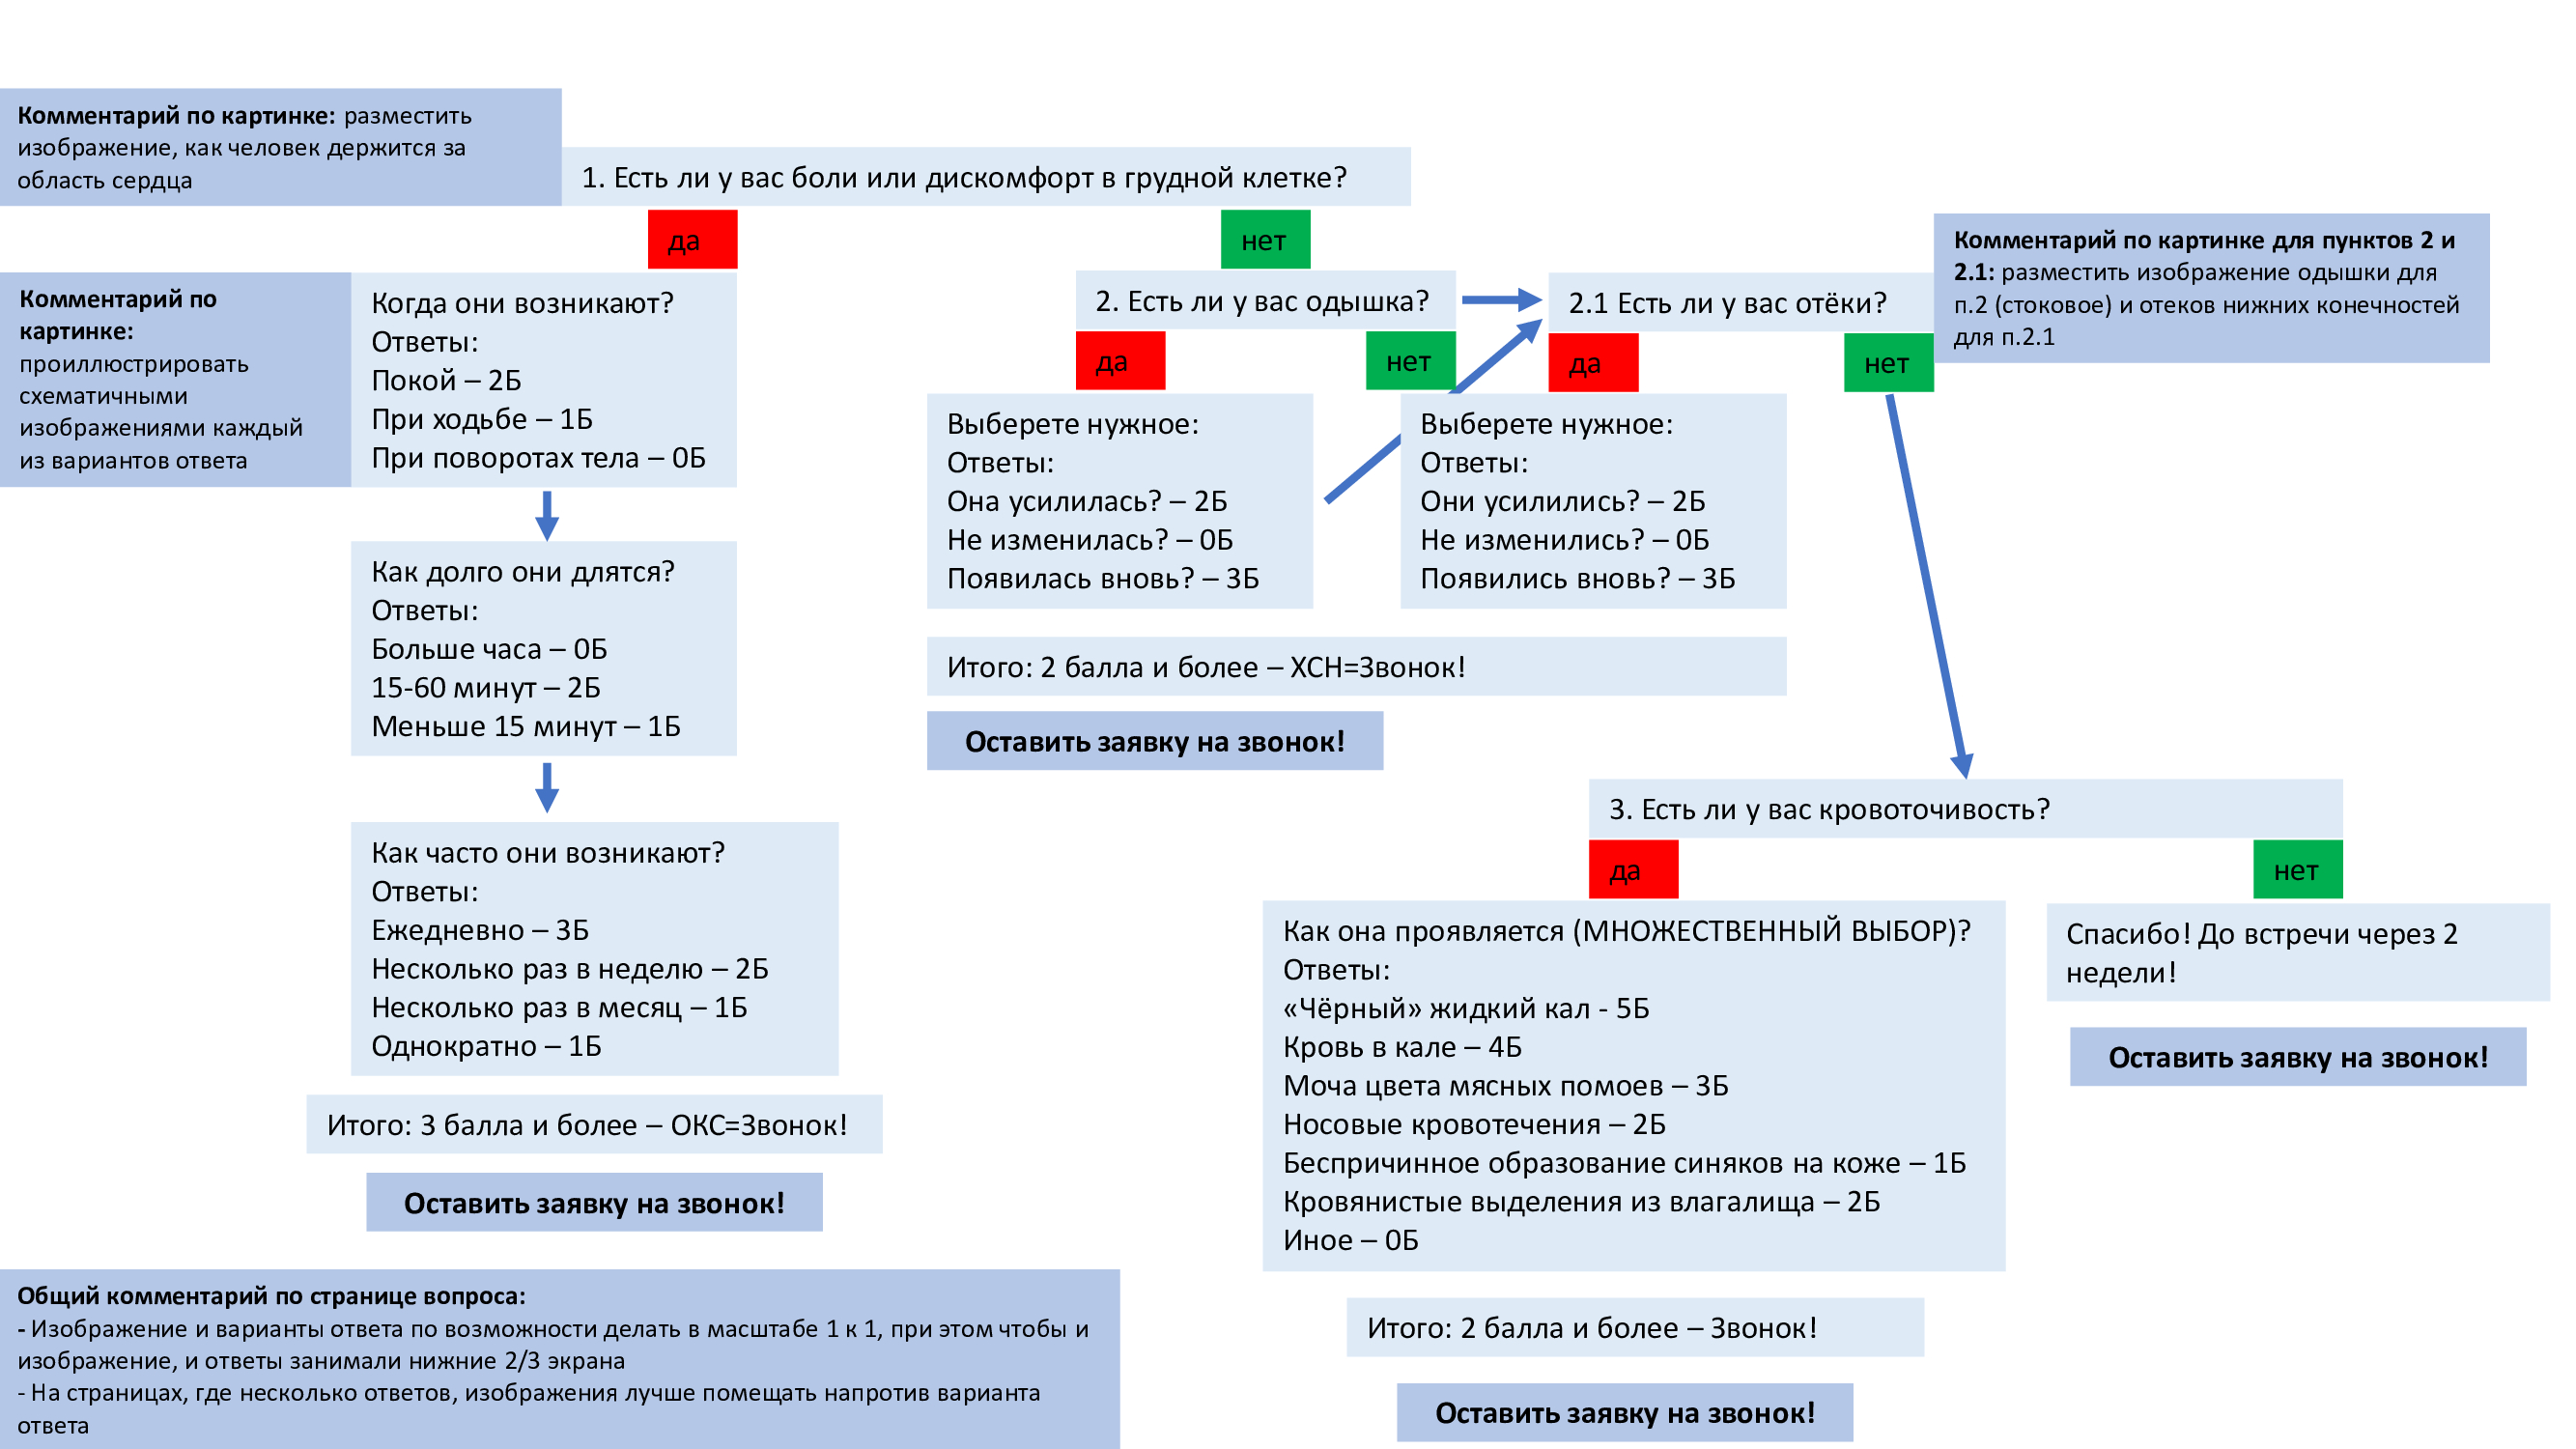
\includegraphics[scale=0.175]{images/presentation/1cbc101521d4d97c799189ce193d279d-0}
    \caption{Структура опроса.}\label{fig:figure}
\end{figure}

К примеру, первым вопросом будет \("\)Есть ли у вас боли или дискомфорт в грудной клетке?
.
При положительном ответе, пациент попадает в блок вопросов, состоящий из 3-х вопросов.
При наборе трех и более баллов за эти 3 вопроса, потребуется консультация с врачом.
В противном случае, консультация на данном этапе не требуется. \par
Если на первый вопрос был дан ответ \("\)Нет,\("\)\, то выдается следующий вопрос, ответ на который определит, показывать вопросы из нового блока, или перейти к следующему.

\subsection{Контроль за приемом лекарств}\label{subsec:---}

Не менее важно контролировать прием всех прописанных лекарств.
Отвечая на вопросы, можно определить, какие из них пациент не принимает, а также узнать саму причину.
Можно определить, какое лекарство вызывает у человека ту или иную реакцию в организме.
Проходить данный опрос предлагается раз в 3 месяца.

\begin{figure}[h]
    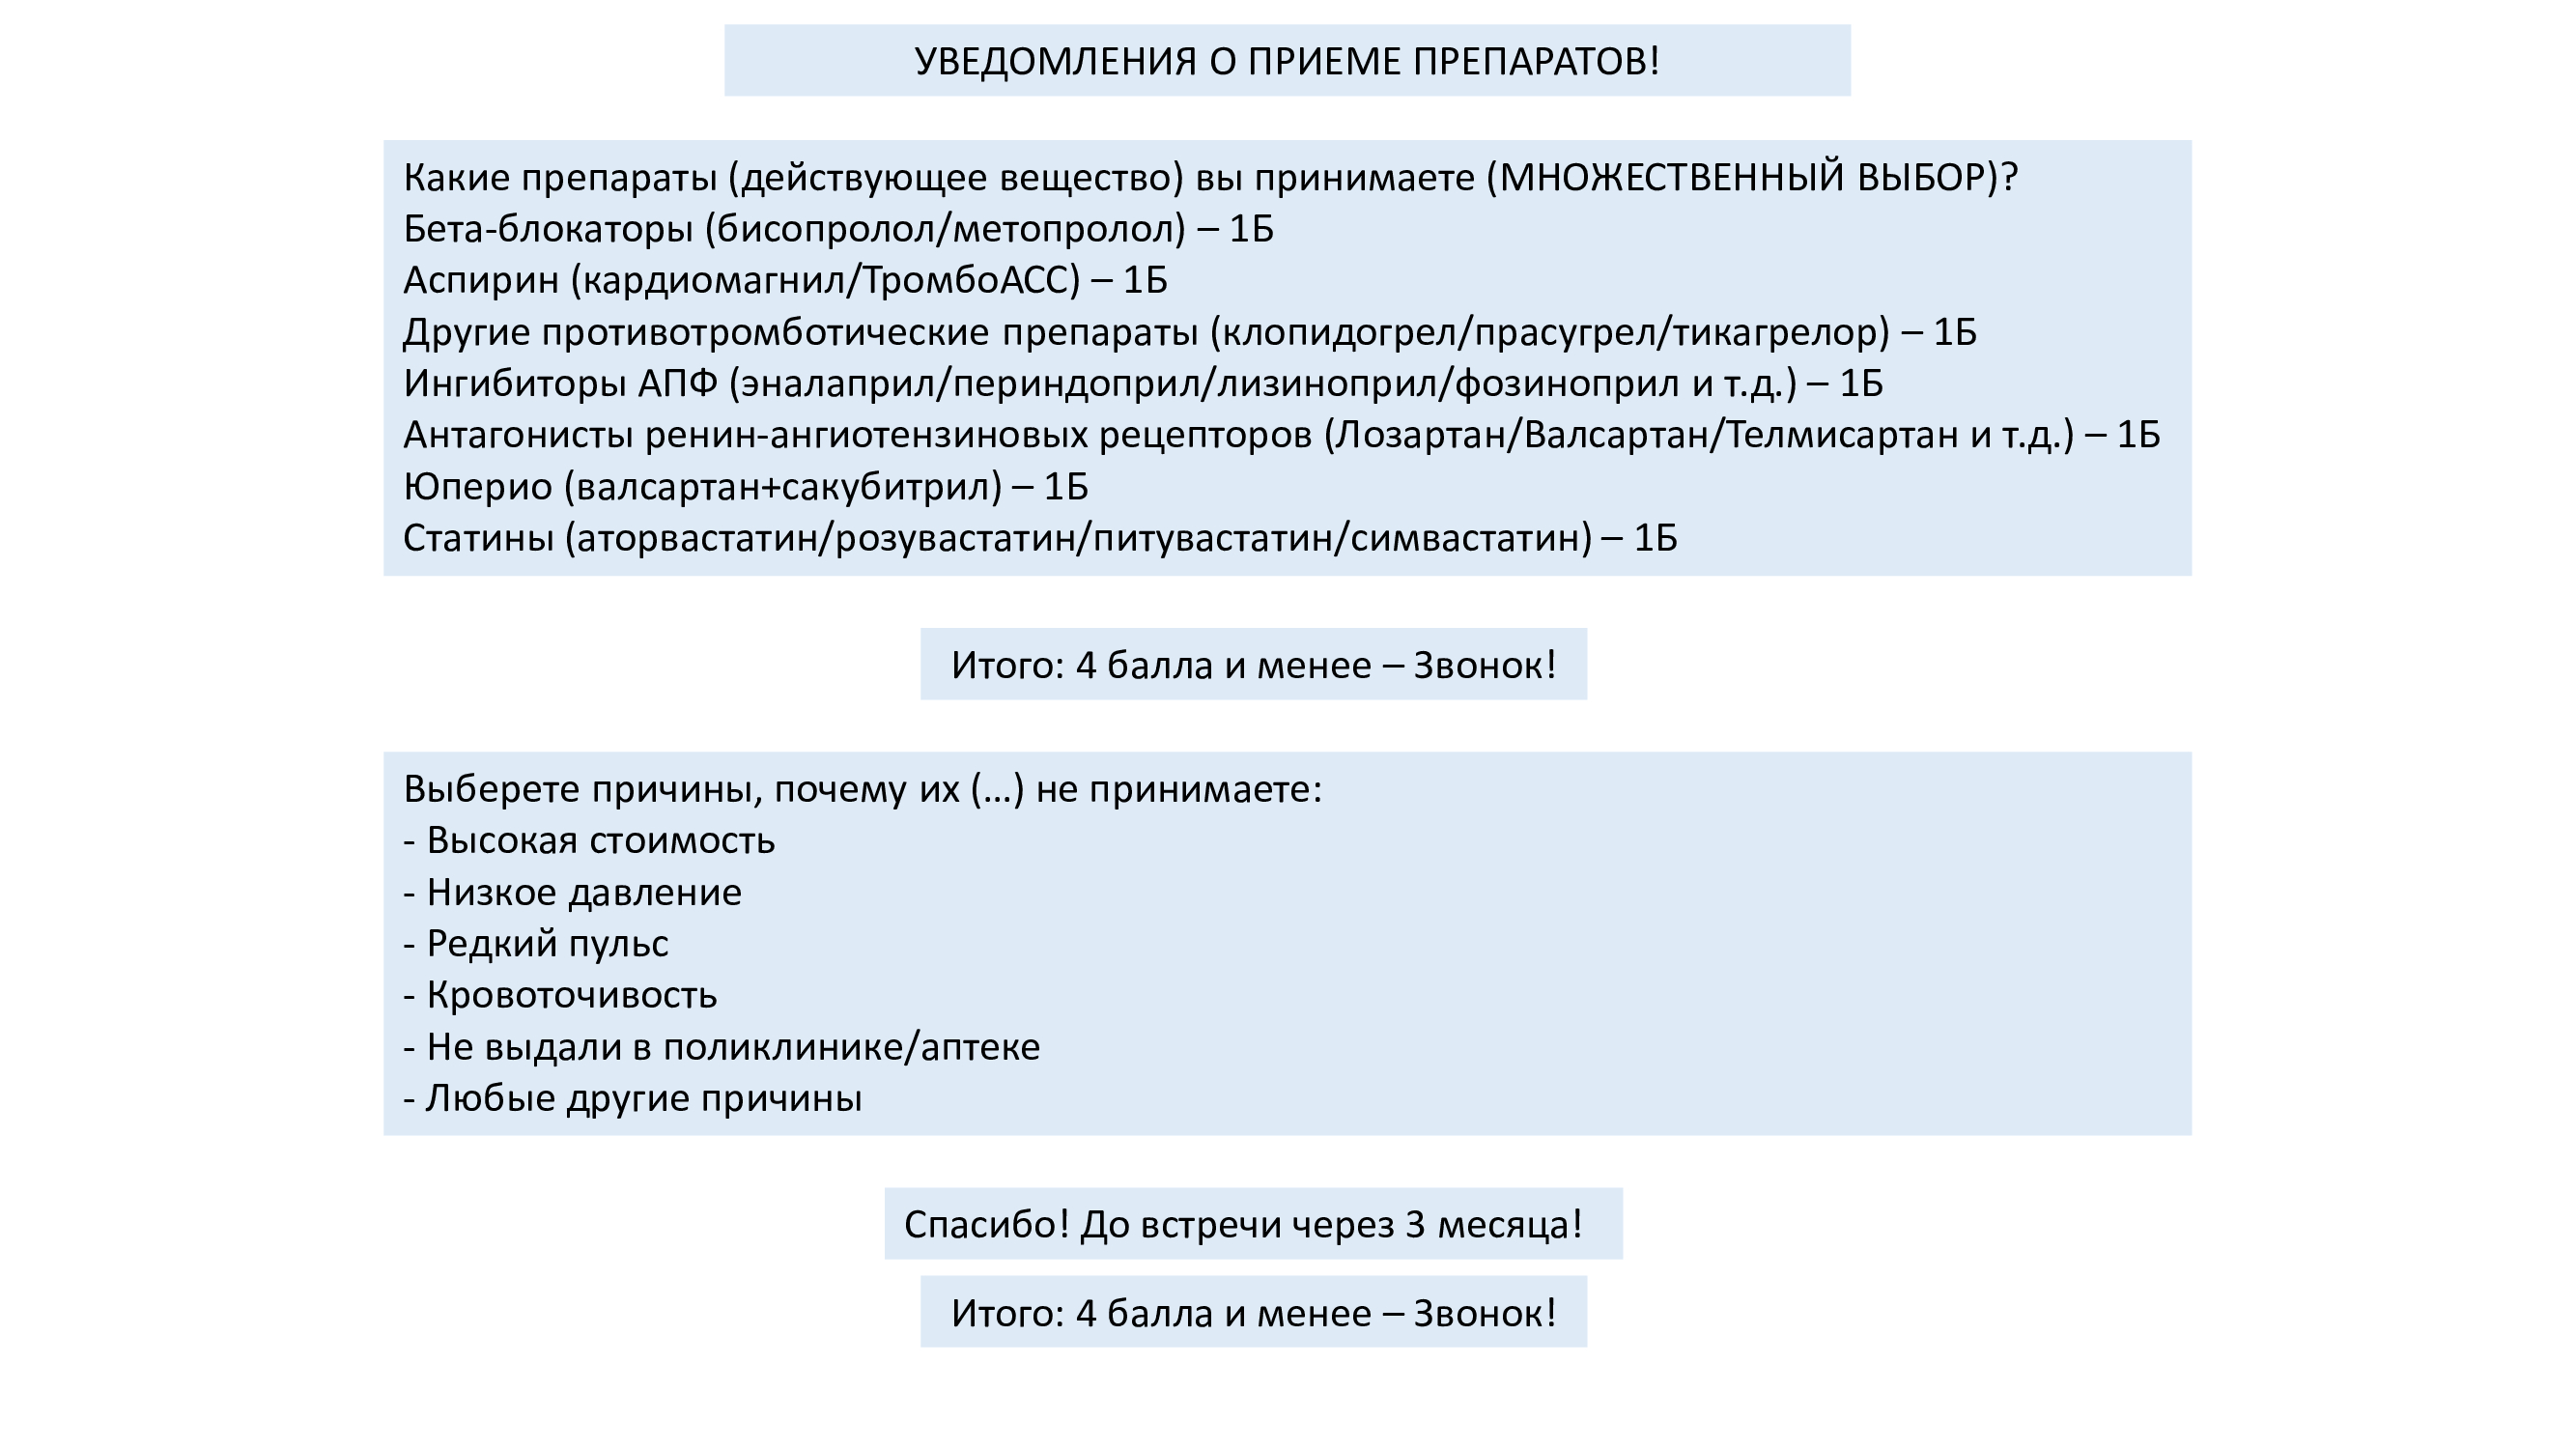
\includegraphics[scale=0.175]{images/presentation/1cbc101521d4d97c799189ce193d279d-1}
    \caption{Опрос лекарства.}\label{fig:figure2}
\end{figure}

\newpage

\subsection{Вредные привычки и физическая активность}\label{subsec:----}

Раз в полгода стоит напоминать пациенту о важности соблюдения режима, о вреде всех его привычек.
Данный опрос предназначен для этого.

\begin{figure}[h]
    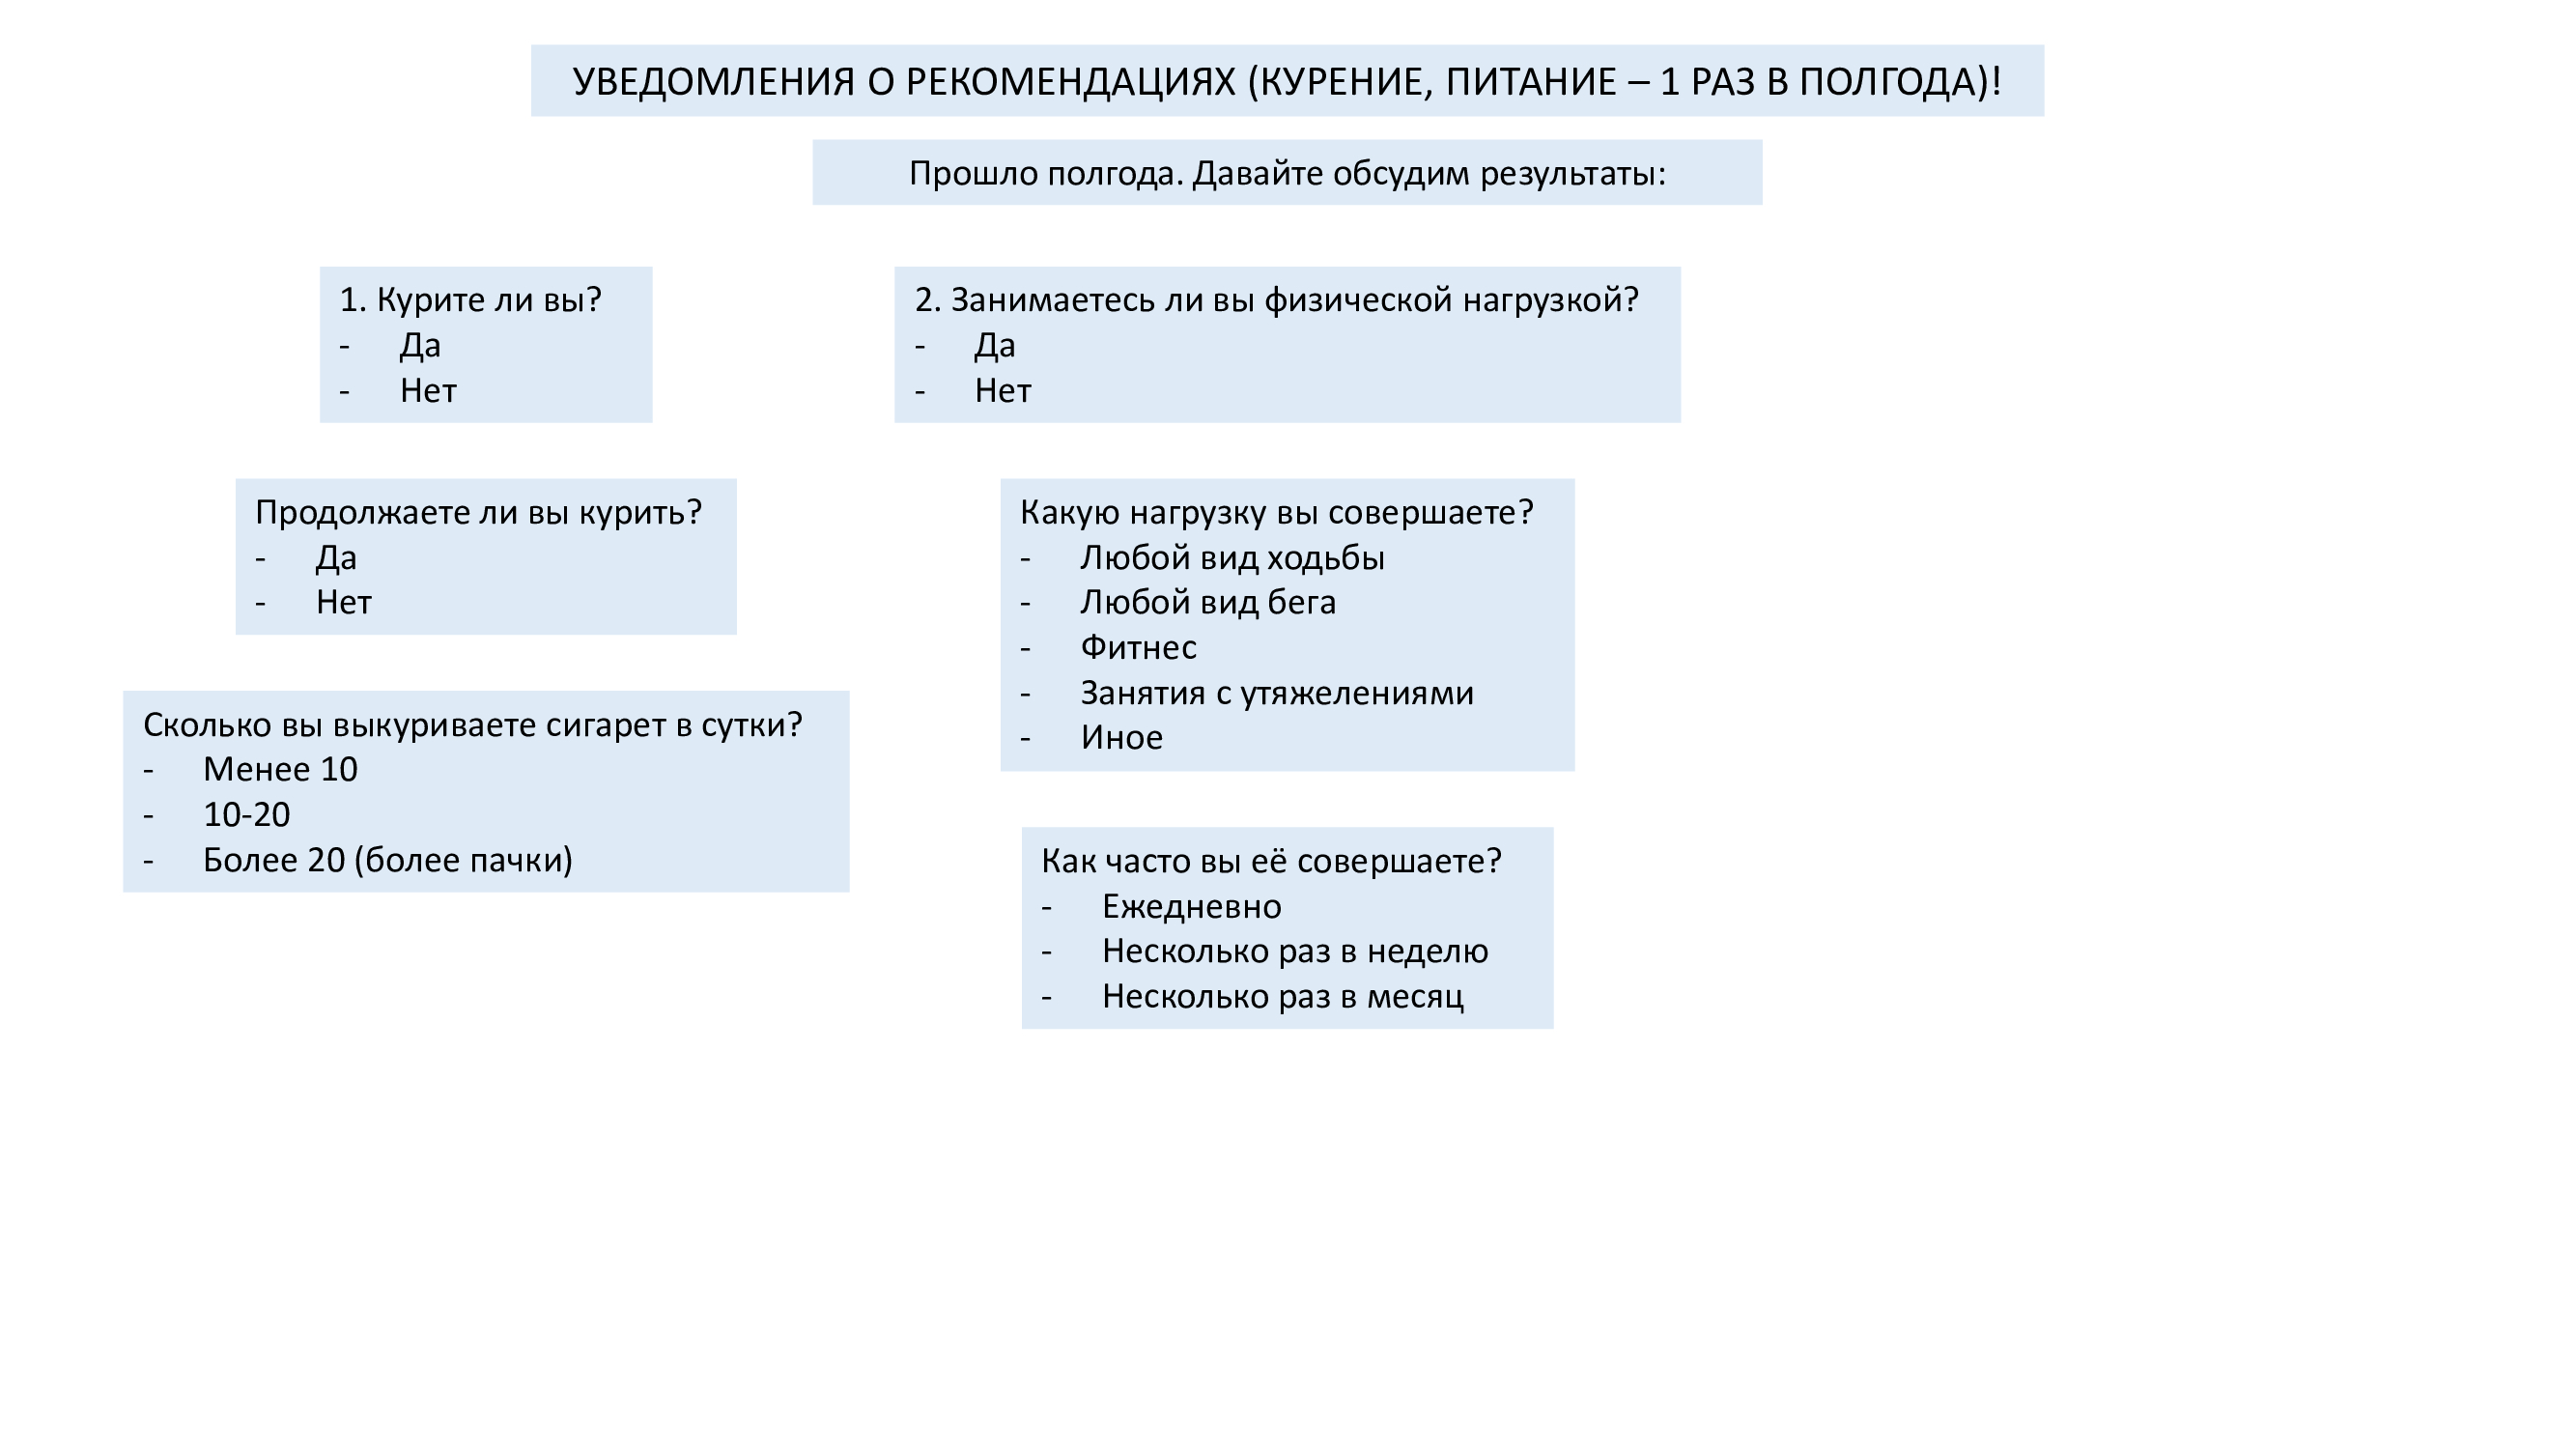
\includegraphics[scale=0.175]{images/presentation/1cbc101521d4d97c799189ce193d279d-2}
    \caption{Рекомендации.}\label{fig:figure3}
\end{figure}